\documentclass[conference]{IEEEtran}
% \IEEEoverridecommandlockouts serve solo a identificare il finanziamento nella prima nota
% del blocco autori (\thanks). Qui il finanziamento sta in \section*{Acknowledgment} e non
% c'e' nessun \thanks, quindi la riga va commentata, come prescrive il template stesso.
%\IEEEoverridecommandlockouts
\usepackage{cite}
\usepackage{amsmath,amssymb,amsfonts}
\usepackage{algorithmic}
\usepackage{graphicx}
\usepackage{textcomp}
\usepackage{xcolor}
\usepackage{hyperref}
\def\BibTeX{{\rm B\kern-.05em{\sc i\kern-.025em b}\kern-.08em
    T\kern-.1667em\lower.7ex\hbox{E}\kern-.125emX}}

% Float placement: with two full-width figures the default parameters strand
% almost a full page. These only relax placement, they do not resize anything.
\setcounter{topnumber}{3}
\setcounter{bottomnumber}{2}
\setcounter{totalnumber}{4}
\renewcommand{\topfraction}{0.95}
\renewcommand{\bottomfraction}{0.7}
\renewcommand{\textfraction}{0.05}
\renewcommand{\floatpagefraction}{0.85}

\begin{document}

\title{Federated TimeVQVAE Anomaly Detection:\\
Prior Sharing Requires an Aligned Tokenizer}

% Sette autori su due affiliazioni: i blocchi per-autore del template (uno per
% \and, tre per riga) costerebbero tre righe di blocchi. La forma compatta e'
% quella a marcatori di IEEEtran (\IEEEauthorrefmark), che tiene l'ORDINE
% originale degli autori e sta dentro il margine. Attenzione: raggruppare i nomi
% per affiliazione, come in una versione precedente, riordina la firma.
\author{
\IEEEauthorblockN{Leonardo Schiavo\IEEEauthorrefmark{1},
Donato Cerciello\IEEEauthorrefmark{1},
\'Angel Panizo-Lledot\IEEEauthorrefmark{1},
Javier Huertas Tato\IEEEauthorrefmark{1},\\
Stefano Izzo\IEEEauthorrefmark{2},
Fabio Giampaolo\IEEEauthorrefmark{2},
David Camacho\IEEEauthorrefmark{1}}
\IEEEauthorblockA{\IEEEauthorrefmark{1}\textit{Departamento de Sistemas Inform\'aticos},
\textit{Universidad Polit\'ecnica de Madrid}, Madrid, Spain\\
\IEEEauthorrefmark{2}\textit{Department of Mathematics and Applications ``R.\ Caccioppoli''},
\textit{University of Naples Federico II}, Naples, Italy}
}

\maketitle

\begin{abstract}
Time series anomaly detection is often carried out by parties that cannot pool their raw data. We
ask what should be shared when the detector is a two-stage generative model: TimeVQVAE-AD first
learns a discrete tokenizer of the signal, then a prior over the resulting tokens. The two stages cannot be federated independently. Sharing the prior
helps only once the clients' tokenizers have been aligned by averaging their encoders, and the
identical change is a null when they have not been, because the prior is indexed by token identity
and unaligned clients use those identities differently. On the UCR anomaly archive, with every
series split across five clients, the federated model improves over local training in the ranking of
anomalous timesteps and matches pooled training on the archive's own localization metric on most
series, a metric on which pooled training, which sees all the data, does not separate from local
training either. We also describe a case in which averaging spreads a false alarm raised by a
minority of the clients to all of them, and show that fusing the local models' scores instead of
their weights avoids it.
\end{abstract}

\begin{IEEEkeywords}
federated learning, time series anomaly detection, vector quantization, generative models,
model aggregation
\end{IEEEkeywords}

\section{Introduction}

Time series anomaly detection~\cite{blazquezgarcia2022review,schmidl2022anomaly} is often performed
where sensors, machines or organizations collect data independently and cannot share their raw
observations~\cite{zhu2022fedexdnn,xu2024pefad}, and federated learning
(FL)~\cite{mcmahan2017federated} exploits that data without centralizing it. On the UCR anomaly
archive~\cite{wu2023ucr} the collaboration is worth having: whenever the methods can be
distinguished, pooled training outperforms the average client, although not necessarily the best
one. We study how to realize it for TimeVQVAE-AD~\cite{lee2024timevqvaead}, a two-stage generative
detector composed of a VQ-VAE~\cite{van2017neural} tokenizer and a masked prior over the resulting
discrete tokens~\cite{lee2023timevqvae}, whose structure raises a question that is less explicit in
end-to-end detectors: which components should be shared, and how should federation of the tokenizer
and of the prior be coordinated?

These decisions turn out not to be separable. Sharing the codebook alone can underperform purely
local training, while federating the encoder, pooling batch normalization (BN) statistics and
aggregating the codebook through sufficient statistics does not improve on the local baseline when
the prior stays local. The strongest configuration combines all of these with a mostly shared prior,
keeping the channel embedding, output bias and decoder local; it matches centralized training
exactly on three of the four development series on which the methods separate at all, and fails on
the fourth, \texttt{ucr\_170}, which we analyze as a failure case. On a pre-registered random sample of
50 further series it improves the ranking of anomalous timesteps over local training on 32 of 48
($p=0.029$ on the area under the precision-recall curve, AUPRC) and matches centralized training
on the archive's own accuracy on 37 of 48,
a metric on which the pre-registered primary endpoint reaches significance for no contrast,
centralized training included, so that what the sample establishes is parity with the pooled upper
bound rather than a gain in localization.

Matched ablations attribute the improvement to prior sharing, but only after the token
representation has been aligned across clients, consistently with the observation that parameter
averaging requires compatible internal
representations~\cite{entezari2022permutation,wang2020fedma}. For a discrete
generative model the requirement is sharper: prior parameters can be shared only when token indices
have common semantics \emph{and} clients map windows to those indices consistently. We contribute a
coordinated federation strategy for such detectors, in which alignment is a measured property of the
checkpoints rather than a label, and a case study of a failure mode of weight-space aggregation
together with a function-space repair that recovers it where it occurs.

\section{Related Work}

\textbf{Federated learning.} FL lets clients train a shared model while their data stay
local~\cite{kairouz2021advances}, with FedAvg as the reference point~\cite{mcmahan2017federated}.
Parameter averaging is brittle when local models drift apart, and the remedies act on the local
objective, the local update or the
server~\cite{li2020fedprox,karimireddy2020scaffold,reddi2021adaptive}, or match internal units
before averaging them~\cite{wang2020fedma}; a second line shares only part of the model, a global
body with personal heads~\cite{arivazhagan2019fedper} or the mirror
arrangement~\cite{liang2020lgfedavg}. In federated time series anomaly
detection, Fed-ExDNN aggregates per-device exemplar modules through constrained clustering, aligning
them before averaging~\cite{zhu2022fedexdnn}, and PeFAD adapts a pre-trained language model,
distilling through a shared synthetic dataset~\cite{xu2024pefad}; in both the aggregated
representation is the terminal one, read directly by a scoring function. To our knowledge no
federated work addresses a pipeline in which a discrete tokenizer produces the symbols consumed by
a second, generative prior; accordingly, we compare the local, pooled and federated versions of
one detector rather than detectors against one another.

\textbf{Discrete tokenization and shared codebooks.} VQ-VAE builds a discrete latent representation
on a learned codebook and fits a prior over the codes in a second stage~\cite{van2017neural};
TimeVQVAE carries this to time series with a Transformer prior~\cite{lee2023timevqvae} and
TimeVQVAE-AD reuses the structure for detection~\cite{lee2024timevqvaead}. The closest analogues to
sharing a codebook transfer knowledge without averaging full weight vectors: federated clustering
of centroids~\cite{dennis2021kfed}, shared prototypes~\cite{tan2022fedproto}, distributed
clustering for globally consistent representations~\cite{lubana2022orchestra}. None of them is a
discrete vocabulary read by a downstream model, so aligning them improves the quality of the
aggregate, not its well-definedness. When the vocabulary is itself federated, alignment becomes a
precondition for prior sharing to be well posed at all.

\section{Background: TimeVQVAE-AD}
\label{sec:background}

We summarize what the federation design needs, referring to the original
paper~\cite{lee2024timevqvaead} for the method; throughout, a \emph{client} owns a set of windows
of a univariate series and never shares them.

Stage~1 is a VQ-VAE~\cite{van2017neural} over the short-time Fourier transform of a window: an
encoder $E$ and a vector quantizer with codebook $\mathcal{C}=\{e_k\}_{k=1}^{K}$ map
$x\in\mathbb{R}^{T}$ to a grid $s\in\{1,\dots,K\}^{H\times W}$ of code indices, which we call
\emph{tokens} and a decoder reconstructs; the convolutional kernels are frequency-independent, so
each token localizes a specific time and frequency region. Stage~2 freezes $E$ and the decoder and
fits a MaskGIT prior~\cite{chang2022maskgit} $p_\theta(s)$ by masked modeling, as in
TimeVQVAE~\cite{lee2023timevqvae}. The second consumes what the first produces: the prior is a
categorical model \emph{over the indices} the first stage emits, and the rows of its output layer
are indexed by that stage's codebook.

% NB: la larghezza della finestra di mascheramento era $\kappa$, lo stesso simbolo dell'accordo
% corretto per il caso di 5.4 (dove kappa e' notazione standard e non si tocca). Qui e' $\ell$.
Detection uses no label. A masking window of odd latent width $\ell$ slides along the temporal
axis of the latent grid, masking whole columns across all frequency bands, and the score of a
latent step is the mean negative log-likelihood the prior assigns to the true tokens of the masked
region. The maps obtained at $\ell=\mathrm{odd}(rW)$ for $r\in\{0.1,0.3,0.5\}$ are summed,
averaged over frequency, mapped back to data space, accumulated over the rolling windows and
averaged with their centered moving average, giving one score per timestep. Two consequences matter
for federation: the score comes from the prior alone, so any choice that touches the tokenizer
reaches detection only through the token grid the prior consumes and the vocabulary it predicts,
and the decoder takes no part in it.

Finally, the coupling between the stages restricts what federation can mean. A token is a pointer
into a codebook, so averaging prior parameters presupposes that index $k$ denotes the same codeword
on every client; and since the index is produced by $E$ and the quantizer jointly, it further
presupposes that clients agree on \emph{which} windows map to $k$. Sharing a dictionary secures the
first condition and not the second.

\section{Federation Design}
\label{sec:design}

Federating TimeVQVAE-AD requires coordinating the tokenizer, which fixes the indices assigned to
each window, and the prior, which models their distribution, so we treat the encoder, the BN
statistics, the codebook and the prior separately; the decoder always stays local, as it does not
contribute to the score. Client $j$ holds $n_j$ training windows and contributes with weight
$\omega_j = n_j/\sum_i n_i$; raw windows never leave the client.
Fig.~\ref{fig:framework} shows the arrangement for configuration (g) below.

\begin{figure}[t]
\centering
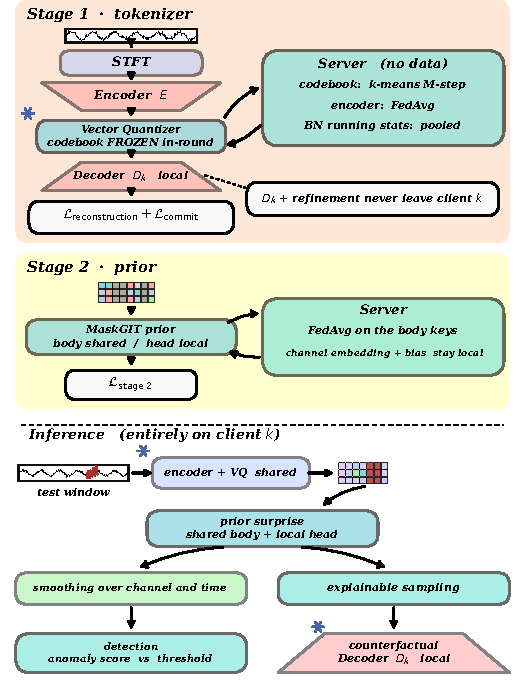
\includegraphics[width=\columnwidth]{fig_framework}
\caption{Configuration (g) on client $k$: the federated components (encoder, BN statistics,
codebook, prior body), the local ones (decoder, prior head) and the local inference fork into
score and counterfactual.}
\label{fig:framework}
\end{figure}

\subsection{Tokenizer federation}
\label{subsec:tokenizer}

The encoder can remain local or be shared through FedAvg~\cite{mcmahan2017federated}; when it is
federated, its BN running statistics are pooled:
\begin{equation}
    \bar{\phi} = \sum_j \omega_j \phi_j, \quad
    \bar{\mu} = \sum_j \omega_j \mu_j, \quad
    \bar{v} = \sum_j \omega_j (v_j + \mu_j^2) - \bar{\mu}^2 .
    \label{eq:bnpool}
\end{equation}
This is the opposite of the FedBN prescription~\cite{li2021fedbn}: here the clients observe the same
sensor and regime, so there is no feature shift for a local BN layer to absorb, while a shared
tokenizer requires that every client normalize identically before quantization.

The codebook can be federated in two ways. Direct FedAvg averages corresponding codewords after
local training, which need not leave the average near any of them once the clients' quantizers have
drifted apart during the round. Our alternative keeps the broadcast codebook fixed during the round
and aggregates assignment statistics: for every code $k$, client $j$ sends its assignment count
$c_{j,k}$ and the sum $m_{j,k}$ of the corresponding pre-quantization encoder vectors, and the
server computes
\begin{equation}
    N = \sum_j c_j, \qquad
    M = \sum_j m_j, \qquad
    e_k = M_k / \tilde{N}_k,
    \label{eq:suffstat}
\end{equation}
with $\tilde{N}_k$ a Laplace-smoothed count, so that each global codeword is updated from per-code
aggregates accumulated across clients. This motivates the
alternative but is not a demonstrated defect of averaging: Section~\ref{subsec:interaction} finds
the two rules indistinguishable in aggregate. Fixing the codebook within a round does not freeze the
tokenizer, since the encoder keeps changing. Neither rule is a privacy mechanism: a code a client
assigns only once sends that latent verbatim under~\eqref{eq:suffstat}, and a formal guarantee
would require secure aggregation on top.
% La frase precedente diceva «without transmitting latent samples or raw data»: falsa nel caso
% limite c_{j,k}=1, dove m_{j,k} E' il latente. Indebolita il 2026-08-16: si afferma
% aggregazione, non privacy.

\subsection{Prior federation}
\label{subsec:coupling}

Prior federation requires a shared vocabulary: the MaskGIT prior predicts codebook indices, so index
$k$ must refer to the same codeword across clients, and averaging prior parameters learned with
independent dictionaries would combine parameters attached to unrelated symbols. We therefore allow
prior sharing only when clients use a common codebook. A common dictionary alone does not guarantee
identical assignments, which also depend on the encoder, so we evaluate prior sharing both with
local encoders and after encoder federation.

We compare a fully local prior with a partially shared one, in which the transformer, the token
embedding, the frequency and time embeddings and the readout are shared while the channel component
of the positional encoding and an additive output bias remain local; on univariate data
personalization therefore acts mainly through the output bias. Stage~2 is aggregated after a fixed
number of local epochs, or, in a variant, after exactly $\tau$ optimizer steps.

\subsection{Evaluated configurations}
\label{subsec:configs}

Table~\ref{tab:space} summarizes the configurations. Two matched comparisons carry the argument: (c) and (e) differ only in prior sharing while
the encoder stays local, and (f) and (g) make the same comparison after encoder federation. The last
two rows replace one stage by its pooled counterpart, so that the two stages can be blamed
separately. Configurations (j) to (m) vary how the
encoder is aggregated at the codebook and prior settings of (f), with
FedProx~\cite{li2020fedprox} acting on the local objective, FedProto~\cite{tan2022fedproto}
broadcasting per-code prototypes, and (m) sharing only the starting point.

\begin{table}[t]
\caption{Configurations evaluated.}
\label{tab:space}
\centering
\scriptsize
\setlength{\tabcolsep}{2.2pt}
\renewcommand{\arraystretch}{1.1}
\begin{tabular}{@{}p{2.2cm}lllllc@{}}
\hline
\textbf{Configuration} & \textbf{Encoder} & \textbf{BN} & \textbf{Codebook} & \textbf{Prior} & \textbf{Stage 2} & $n$ (disc.) \\
\hline
(a) local & local & --- & local & local & --- & 10 (4/4) \\
(b) centralized & \multicolumn{5}{c}{one model on the pooled windows (reference)} & 10 (4/4) \\
\hline
(c) codebook only & local & --- & suff.\,stat. & local & --- & 10 (4/4) \\
(d) codebook only, averaged dictionary & local & --- & FedAvg & local & --- & 10 (4/4) \\
(e) codebook and shared prior body & local & --- & suff.\,stat. & partial & epochs & 10 (4/4) \\
(f) aligned tokenizer, local prior (A1) & FedAvg & pooled & suff.\,stat. & local & --- & 10 (4/4) \\
(g) aligned tokenizer, shared prior body (A2) & FedAvg & pooled & suff.\,stat. & partial & epochs & 10 (4/4) \\
(h) (g) with a step-counted rhythm & FedAvg & pooled & suff.\,stat. & partial & $\tau$ steps & 10 (4/4) \\
(i) (h) with a mobile dictionary & FedAvg & pooled & FedAvg & partial & $\tau$ steps & 3 (3/4) \\
\hline
\multicolumn{7}{@{}l@{}}{\emph{Encoder aggregation rule, isolated at a local prior}$^{\mathrm{b}}$} \\
(j) encoder FedAvg, local BN stats & FedAvg & affine & suff.\,stat. & local & --- & 10 (4/4) \\
(k) (j) with FedProx & FedProx & affine & suff.\,stat. & local & --- & 10 (4/4) \\
(l) (j) with FedProto & prototypes & init & suff.\,stat. & local & --- & 10 (4/4) \\
(m) (j) with a shared initialization only & init & init & suff.\,stat. & local & --- & 10 (4/4) \\
\hline
(n) score fusion$^{\mathrm{a}}$ & local & --- & local & local & --- & 10 (4/4) \\
\hline
\emph{pooled tokenizer}$^{\mathrm{c}}$ & \multicolumn{5}{c}{\emph{pooled stage 1, federated stage 2}} & 1 (1/4) \\
\emph{pooled prior}$^{\mathrm{c}}$ & \multicolumn{5}{c}{\emph{federated stage 1 of (g), stage 2 on pooled tokens}} & 4 (4/4) \\
\hline
\multicolumn{7}{@{}p{8.45cm}@{}}{``FedAvg'' is count-weighted parameter averaging, ``pooled'' the BN aggregation~\eqref{eq:bnpool}, ``suff.\,stat.'' the codebook update~\eqref{eq:suffstat}, ``partial'' the prior with client-specific components local. $n$ = development series run and, in parentheses, coverage of the four that separate the arms at all (Section~\ref{subsec:discriminating}). $^{\mathrm{a}}$Trained exactly as (a); only inference differs. $^{\mathrm{b}}$Rows (j) to (m) target the same encoder parameter tensors as (f) but keep the BN running statistics local (``affine'' shares BN scale and shift every round, ``init'' only at initialization), so they are matched to one another and \emph{not} to (f), (g) and (h): their baseline is (j). FedProx uses $\mu=0.01$; (m) is (l) with the prototype pull set to zero. $^{\mathrm{c}}$Not federation-legal, diagnostic only. \emph{Pooled prior} runs on exactly the four discriminating series, so its $n=4$ covers the informative subset completely. Both are matched to the reference of Section~\ref{subsec:main}, not to (g).}
\end{tabular}
\end{table}

\subsection{Score fusion}
\label{subsec:fusion}

As an alternative to parameter sharing we also combine independently trained local models at
inference time, as outlier ensembles~\cite{kriegel2011unifying,aggarwal2015outlierensembles} and
function-space federated aggregation~\cite{lin2020feddf} do: each client keeps its tokenizer and
prior unchanged, computes its profile and
standardizes it over time, and the final score is the pointwise mean across clients, so that only
per-timestep score vectors are combined and no alignment of parameters, codewords or indices is
needed. No training is shared; the profiles can be averaged only because the split divides the
training segment while the test segment is common, and all five models must be present at
inference: neither holds where clients score their own streams.
We also report the median, the trimmed mean and the mean of normalized ranks.

\section{Experimental Protocol}
\label{sec:protocol}

\subsection{Benchmark, choice of series and split}

\begin{figure*}[t]
\centering
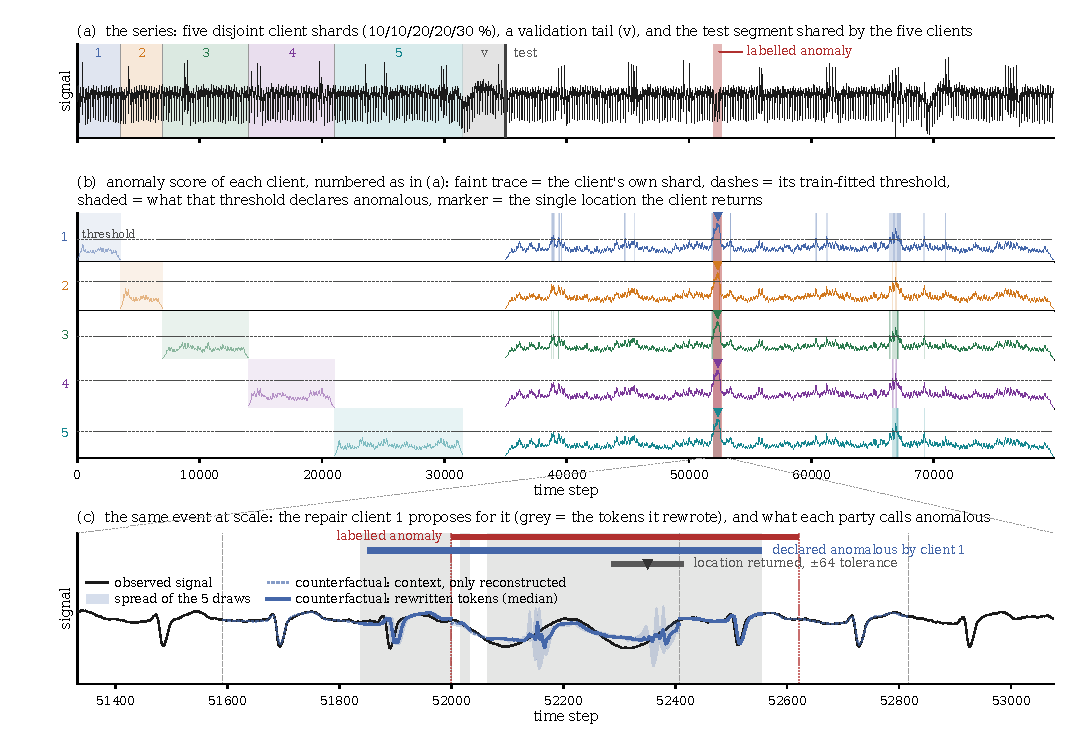
\includegraphics[width=\textwidth]{fig_overview}
\caption{\texttt{ucr\_001} under configuration (g): (a)~the split, (b)~each client's score, threshold
and returned location, (c)~the labelled event with the counterfactual of client~1. The reading key is
in the panel headings.}
% «Every configuration already localizes this series» tolta il 2026-08-16 per il tetto delle 8
% pagine: la stessa informazione sta in VI-A (local gia' a 1.00 su ucr_001).
\label{fig:overview}
\end{figure*}

Two settings are inherited from the original method rather than tuned, since it states them as
such: the window length is $T=2P$, twice the tabulated period of the series, and each input window
is z-normalized before the transform; its frequency resolution is kept as well
(Table~\ref{tab:hparams}). With $T=2P$ the UCR Time Series Anomaly archive~\cite{wu2023ucr} leaves
180 usable series: the remainder are too short at that window to give every client shard two
windows, the validation tail one and the test segment two.
Ten form a development set on which the configurations were
% Criterio allineato a build_ucr_split.py (min client 2W, min val 1W, min test 2W): la vecchia
% frase «fewer samples than one window» era una semplificazione falsa ai bordi.
explored, selected by period and domain rather than by detection performance, with window lengths
roughly log-spaced from $182$ to $970$ samples.
A disjoint set of 50 was then drawn uniformly at random with a fixed seed
from the remaining 170, the same draw fixing their execution order; the sample, its order, the three
configurations run on it, the primary metric, the stopping rule, a minimum sample size and a freeze
date were all fixed before observing any of its results
(Section~\ref{subsec:confirmation}).

Each series is an independent federated task: no parameter, statistic or window is shared between
series. Within a series the training segment is divided chronologically among five clients holding
$10\%$, $10\%$, $20\%$, $20\%$ and $30\%$ of the data, the final $10\%$ is held out for validation,
and the archive's test segment and labels are never used in training (Fig.~\ref{fig:overview},
where the five clients of (g) all localize the event while their thresholds admit $1.2$ to $4.1\%$
of the test timesteps).
Windows are extracted with unit stride, so a shard of length $L$ contributes $L-T+1$ windows, and
these counts are the aggregation weights of Section~\ref{sec:design}. The split is deliberately
homogeneous: the five clients observe the same sensor, regime and units and differ only in how
much of the series they hold. This removes client heterogeneity as the intended explanation for
differences between local and federated training.

\subsection{Training}

All configurations use the trainer of Table~\ref{tab:hparams} and select the best validation round;
the criteria differ only in their unit, optimizer steps for local and centralized training and
aggregation rounds for federated ones, and a federated stage whose best round is its last is
reported as truncated. The baselines' step ceiling binds in $21\%$ of their stage-runs on the
development set and in $15$ to $25\%$ on the confirmation sample, and those runs are retained, so
the baselines are, if anything, the arm more likely to be reported before convergence.

Capacity is fixed across configurations, with a codebook smaller than in the original method, so
our reference results are not directly
comparable with its published accuracy. One seed is run per experimental cell. We also
report a parameter-free floor, the squared residual of a centered moving average of length $10$
pushed through the same detection path; having no parameters it admits no federated variant and is a
lower reference, not a competitor.

\subsection{Metrics and unit of analysis}

We report the archive's accuracy, where a method returns one predicted location per series and is
correct within $64$ timesteps of the labelled anomaly, and the AUPRC of the per-timestep score. The
two are not interchangeable: the archive metric is the benchmark's own, so it leaves us no
discretion, and it is correspondingly coarse, one hit or miss per series; AUPRC is ours and uses the
whole profile. We do not report the area under the ROC curve (AUROC), which saturates here (it
exceeds $0.95$ on 8 of 48
confirmation series for a configuration whose predicted location misses the anomaly entirely), nor
threshold-based scores: the train-fitted threshold, a sum over rates of per-rate train quantiles,
leaves nothing of the training profile above it at the nominal $q=0.99$ and admits between $0.000$
and $0.978$ of the test timesteps depending on the arm, nor range-aware measures~\cite{paparrizos2022vus}, whose scale
depends on anomaly duration. The unit of analysis is the series: the five clients are shards of one
signal, not independent replicates, so comparisons are paired by series.

\subsection{Implementation details and reproducibility}
\label{subsec:repro}

Table~\ref{tab:hparams} lists the settings shared by every configuration, as recorded in the launch
metadata of the runs. The code, one command per row of Table~\ref{tab:space}, the cohort files, the
pre-registration and the per-cell results are available~\cite{schiavo2026fedtimevqvae}, with a
checker for every number below that needs no checkpoint.

\begin{table}[t]
\caption{Settings shared by all configurations.}
\label{tab:hparams}
\centering
\scriptsize
\setlength{\tabcolsep}{2.2pt}
\renewcommand{\arraystretch}{1.0}
\begin{tabular}{@{}l p{6.95cm}@{}}
\hline
data & window $T=2P$, twice the period of the series; per-window z-score; unit stride; five client shards at $10/10/20/20/30\%$ of the training segment, its last $10\%$ for validation \\
tokenizer & STFT with $n_\mathrm{fft}=4$, giving $H=3$ frequency bands; encoder of base width $16$ with BN; codebook of $K=64$ entries of dimension $64$, EMA $0.99$ \\
prior & MaskGIT with $4$ layers, $4$ heads, width $128$, feed-forward $512$, dropout $0.2$, cosine mask schedule \\
optimization & AdamW, learning rate $10^{-3}$, weight decay $0.01$, batch $64$, fp16 mixed precision; the baselines warm up over $10\%$ of their step ceiling and then decay by cosine, the federated rounds run at constant rate \\
stopping & baselines: patience $2000$ steps within a ceiling of $10^4$ (stage 1) and $5000$ within $5\times10^4$ (stage 2); federated: $10$ local epochs per round, patience $6$ rounds, ceiling $300$ rounds per stage \\
variants & (h) and (i): $\tau=64$ optimizer steps per round, stage-2 patience $29$ rounds, stage~1 taken from (g); (k): FedProx $\mu=0.01$ \\
scoring & $\ell=\mathrm{odd}(rW)$ summed over $r\in\{0.1,0.3,0.5\}$; detection windows at stride $\mathrm{round}(0.1\,T)$; the score averaged with its centered moving average of length $T$; threshold at the train quantile $q=0.99$; archive tolerance $64$ \\
runs & one seed ($0$) per cell; the confirmation sample drawn with seed $20260809$; trained on RTX~3090, RTX~4500~Ada and Quadro~RTX~8000 GPUs \\
\hline
\end{tabular}
\end{table}

\section{Results}
\label{sec:results}

Results are from the ten-series development set unless stated otherwise, one seed per cell, with
client-level results averaged to one value per series.

\subsection{Which series can separate the methods}
\label{subsec:discriminating}

Local training already scores $1.00$ on \texttt{ucr\_001}, \texttt{ucr\_083} and \texttt{ucr\_086},
leaving no room for improvement, and both local and centralized training score $0.00$ on
\texttt{ucr\_082}, \texttt{ucr\_222} and \texttt{ucr\_229}, which therefore carry no evidence about
federation. The remaining four, \texttt{ucr\_011}, \texttt{ucr\_014}, \texttt{ucr\_043} and \texttt{ucr\_170},
are the informative cases for the archive metric, and on four series a two-sided sign test cannot
reach $p<0.05$ (its minimum attainable value is $0.125$), so we
emphasize per-series magnitudes and win/loss counts rather than significance.

\subsection{Reference points}
\label{subsec:reference}

Pooling all client windows improves over the average local model on 9 of 10 series in AUPRC and on
all four discriminating series in the archive metric, where local training obtains $0.40$, $0.80$,
$0.20$ and $0.20$ against $1.00$ for centralized training in every case. Against the best individual
client, $\max_j$, the picture differs: centralized training exceeds it on 7 of 10 series in AUPRC ($p=0.34$),
but on the archive metric never detects an anomaly that no individual client detects, the two
scoring identically on all ten series, and $\max_j$ is an oracle either way.
The parameter-free floor stays far below all of them, median AUPRC $0.007$
against $0.353$ for local and $0.899$ for centralized training, and is exceeded by every trained arm
on all ten series, though on \texttt{ucr\_083} it reaches $0.825$, consistent with that series
being uninformative about federation.

\subsection{Main federated configuration}
\label{subsec:main}

Configuration (g) reaches the centralized archive score on three of the four discriminating series
and fails on the fourth (Table~\ref{tab:main}): three improvements, one degradation and six ties, all
six on the non-discriminating series. In AUPRC it improves nine series and degrades one, the gains
concentrated on three ($+0.42$, $+0.46$, $+0.30$) and six of them below $0.036$. Against centralized
training it reaches the same archive score on 9 of 10 series and falls below only on
\texttt{ucr\_170}, while in AUPRC it stays below on 8 of 10: equal localization does not imply equal
ranking of the full profile.

The comparison with local training depends on where local training is stopped. Against the baseline
used throughout, which stops on validation patience, federation improves 9 of 10 series in AUPRC
(sign test $p=0.021$); against a baseline trained to a much larger budget with early
stopping disabled, the median difference is essentially unchanged ($+0.022$ against $+0.021$) but
the count falls to 6 against 4
($p=0.75$), the longer-trained baseline being not uniformly better but more variable: federation
improves local training stopped at its own criterion, not at any budget.

The stage-2 synchronization rhythm, by contrast, is a null on both sets. Replacing epoch-based
rounds with $\tau=64$ optimizer steps at an identical stage~1 checkpoint improves four development
series and degrades six (median $-0.001$); the reference there is not the (g) of
Table~\ref{tab:main} but the arm sharing (h)'s low-noise stage-2 validation oracle, frozen masks in
fp32, which small $\tau$ requires and which changes the round selected, not the trajectory. On the
confirmation sample that arm was not run, so (h) is compared with (g) and the oracle travels with
$\tau$: from the bit-identical stage~1 of (g) it wins 25 against 23 in AUPRC (median $0.0000$,
$p=0.89$) and 2 against 4 with 42 ties on the archive metric ($p=0.69$). Markedly less frequent
aggregation, $24$ and $31$ local epochs per round against the same reference, costs $0.198$ and
$0.245$ AUPRC on \texttt{ucr\_011} and \texttt{ucr\_043}: the default frequency is sufficient.

\begin{table}[t]
\caption{Development set: archive accuracy and AUPRC.}
\label{tab:main}
\centering
\scriptsize
\setlength{\tabcolsep}{2.2pt}
\renewcommand{\arraystretch}{1.1}
\begin{tabular}{@{}l cccc c ccccc@{}}
\hline
& \multicolumn{4}{c}{\textbf{accuracy@64}} & & \multicolumn{5}{c}{\textbf{AUPRC}} \\
\cline{2-5}\cline{7-11}
\textbf{series} & local & $\max_j$ & centr. & (g) & & floor & local & $\max_j$ & centr. & (g) \\
\hline
\texttt{ucr\_011} & 0.40 & 1.00 & 1.00 & \textbf{1.00} & & 0.092 & 0.403 & 0.997 & 0.976 & 0.820 \\
\texttt{ucr\_014} & 0.80 & 1.00 & 1.00 & \textbf{1.00} & & 0.003 & 0.639 & 0.902 & 0.964 & 0.939 \\
\texttt{ucr\_043} & 0.20 & 1.00 & 1.00 & \textbf{1.00} & & 0.046 & 0.181 & 0.819 & 0.875 & 0.637 \\
\texttt{ucr\_170} & 0.20 & 1.00 & 1.00 & 0.00 & & 0.015 & 0.303 & 0.588 & 0.878 & 0.086 \\
\hline
\texttt{ucr\_001} & 1.00 & 1.00 & 1.00 & 1.00 & & 0.007 & 0.820 & 0.903 & 0.920 & 0.851 \\
\texttt{ucr\_083} & 1.00 & 1.00 & 1.00 & 1.00 & & 0.825 & 0.922 & 0.983 & 0.932 & 0.932 \\
\texttt{ucr\_086} & 1.00 & 1.00 & 1.00 & 1.00 & & 0.007 & 0.938 & 0.979 & 0.986 & 0.973 \\
\texttt{ucr\_082} & 0.00 & 0.00 & 0.00 & 0.00 & & 0.000 & 0.000 & 0.000 & 0.000 & 0.000 \\
\texttt{ucr\_222} & 0.00 & 0.00 & 0.00 & 0.00 & & 0.002 & 0.046 & 0.077 & 0.083 & 0.054 \\
\texttt{ucr\_229} & 0.00 & 0.00 & 0.00 & 0.00 & & 0.002 & 0.002 & 0.003 & 0.018 & 0.005 \\
\hline
\multicolumn{11}{@{}p{7.6cm}@{}}{Above the rule, the four discriminating series. $\max_j$ = best individual client, selected with test labels. On \texttt{ucr\_082} every arm is at floor: the counts in the text rest on differences in the fifth decimal.} \\
\end{tabular}
\end{table}

\subsection{Attribution of the improvement}
\label{subsec:interaction}

To isolate prior sharing we apply the same modification under two tokenizer configurations: (c)
versus (e) with a shared codebook but local encoders, and (f) versus (g) after encoder federation,
the set of shared prior tensors being identical in the two ($55$ keys, with the channel embedding
and output bias local). With the aligned tokenizer, prior sharing improves 9 of 10 series in AUPRC
(median $+0.069$) and all four discriminating series in the archive metric; with local encoders it
gives 4 improvements and 6 degradations (median $-0.001$) and splits 2 against 2. The difference is
positive on 8 of 10 series in AUPRC (median $+0.136$) and on all five non-tied series in the archive
metric: prior sharing is beneficial only after encoder alignment.

``Alignment'' is not a label we attach to the federated arm: it is a property of the checkpoints. We
encode the same validation windows with each client and measure how often two clients assign the
same latent position to the same code, corrected for chance agreement. Under (g) the five clients
tokenize \emph{identically}, $\kappa=1.00$ on every one of the ten series, whereas under (e), whose
encoders are local, the median is $\kappa=0.07$. The
codebook is bit-identical across clients in both arms, so what separates them is not the vocabulary
but whether they use it the same way, exactly the condition a prior indexed by code identity
requires. The same measurement locates the intermediate mechanisms: encoder FedAvg alone reaches
$\kappa=0.77$ under the BN regime of (j), and pooling the BN running statistics, the only remaining
difference, carries it to $1.00$, while (m), which shares the initialization and never averages
again, sits at $\kappa=0.04$, indistinguishable from (e) at $0.07$. A common starting point does not
survive local training; federating the encoder does not make the tokenizers better, it makes them
agree.

What is shared matters more than how it is averaged. Relative to (j), the same FedAvg under the same
BN regime, replacing encoder FedAvg by FedProx, by FedProto or by a control sharing only the
initialization moves the median AUPRC by $-0.004$ (3 wins), $-0.004$ (4 wins) and $-0.000$ (4 wins):
even the control that never communicates ties both algorithms. The codebook rule is equally
uninformative in aggregate but for the opposite reason:
(c) against (d) is five wins each with median $+0.000$ AUPRC, yet the per-series differences
$(c)-(d)$ run from $-0.946$ to $+0.292$, and after alignment the mobile dictionary of (i) loses
$0.063$ and $0.375$ AUPRC against (h) on \texttt{ucr\_011} and \texttt{ucr\_043} while gaining
$0.270$ on \texttt{ucr\_170}, the one series
on which the frozen dictionary is the binding constraint. It is a null of large differences that
cancel, so we fix it to sufficient
statistics and do not present that choice as a contribution.

\subsection{Failure case and score fusion}
\label{subsec:failure}

\texttt{ucr\_170} is the only discriminating series on which the main federated configuration fails
to recover the local baseline. The five local models obtain AUPRC $0.004$, $0.223$, $0.329$, $0.588$
and $0.370$, with mean pairwise score-profile correlation $0.56$; after federation they become
$0.087$, $0.094$, $0.088$, $0.073$ and $0.088$ while the correlation rises to $0.98$. The clients
become far more similar, but the common profile ranks a false alarm above the true anomaly, which
the centralized model contains as well and ranks below it. The diagnostic configurations locate the
responsibility: replacing only the prior of (g) by one fitted on the pooled token grids raises AUPRC
to $0.948$, $0.947$, $0.900$ and $0.202$ on the four discriminating series against $0.870$, $0.944$,
$0.746$ and $0.082$ for the matched federated reference, reaching the centralized level everywhere
but on \texttt{ucr\_170}; both diagnostics share the oracle of Section~\ref{subsec:main}, so their
matched reference is that arm and not the (g) of Table~\ref{tab:main}. Replacing
instead only the tokenizer by a pooled one recovers
\texttt{ucr\_170} to $0.578$: on most series the binding constraint is the prior, on
\texttt{ucr\_170} the order reverses. Both rest on at most four series and one seed and are bounds,
not methods.

Combining the original local models at the score level does much better here. Averaging their
standardized profiles gives AUPRC $0.698$ against $0.086$ for the weight-aggregated model trained on
the same shards, and above the best individual client at $0.588$. Across the ten series the fusion
beats the per-client mean on 7 (median $+0.027$) but the best client only here, where the clients
are the least correlated of the ten ($0.56$ against a median $0.86$). Against (g) it loses 3 to 7
in AUPRC (median $-0.006$), the large losses on the three where prior sharing pays ($-0.53$,
$-0.39$, $-0.23$), and is level on the archive metric (one win, one loss, eight ties), the endpoint that
separates no pair of arms.
The gain depends on the rule and lives in the
amplitude of the peaks rather than their ordering: the trimmed mean gives $0.690$, while the median
and the mean of normalized ranks fall to $0.363$ and $0.277$. Applying it to the federated clients
changes nothing ($0.087$ against $0.086$), their profiles being already nearly identical. Fusion is
therefore a repair for this failure mode, not a detector that supersedes federation.

\subsection{Confirmation on the random sample}
\label{subsec:confirmation}

The pre-registered
sample tests whether the surviving claims hold out of sample, and its analysis was fixed before any
of its numbers existed: the primary endpoint is the archive accuracy at tolerance $64$, compared by
a two-sided paired sign test with ties excluded, and AUPRC is secondary. Three configurations are run
on it: local, centralized and (g).

Of the fifty series, 48 are analyzed: on \texttt{ucr\_190} and \texttt{ucr\_240} the federated arm
aborted on non-finite entries in the aggregated codebook, a non-finite latent entering the
sufficient statistics of~\eqref{eq:suffstat} and one coordinate propagating through the one-hot
reduction to almost every codeword. It is not codebook collapse, and the failure tracks
half-precision training exposure rather than detection difficulty. The pre-registered rule discards
a series from \emph{all} arms when any arm is incomplete; both sit at floor for the reference arms
on the primary endpoint, and recovering both as wins would move the primary contrast against local
training only from $p=0.33$ to $p=0.17$.

Reported in the fixed order, primary endpoint first: \emph{none of the three contrasts reaches
$p<0.05$ on the pre-registered primary endpoint} (Table~\ref{tab:c50}). The reason is in the tie
counts rather than in the effect: a series contributes only when the arms disagree about whether the
single predicted location is found, and they agree on 31 of 48 series for the first contrast and 37
of 48 for the third, so the effective sample size is 17 and 11, not 48. This is a property of the
endpoint and not of federation, and the pooled model is the evidence: centralized training sees
every client's data and still does not separate from local training here.

On the secondary endpoint the picture is the one the development set showed, and it is significant:
in AUPRC centralized training improves on local training on 35 of 48 series ($p=0.002$) and (g) on 32
of 48 ($p=0.029$), while (g) remains below centralized training on 31 of 48 ($p=0.06$). The tension
between the two metrics is therefore not an artifact of a purposive choice of series: it reproduces
on a random sample five times larger. Out of sample, the defensible statement is that federated and
pooled training both improve the ranking of anomalous timesteps over the typical client, and that
neither is shown to improve the archive's own localization accuracy.

\begin{table}[t]
\caption{Confirmation sample ($n=48$), paired by series.}
\label{tab:c50}
\centering
\scriptsize
% 4pt sforavano la colonna di 9,8pt (18 gutter x 4pt = 72pt di tabcolsep)
\setlength{\tabcolsep}{2.5pt}
\renewcommand{\arraystretch}{1.1}
\begin{tabular}{@{}l cccc c ccc@{}}
\hline
& \multicolumn{4}{c}{\textbf{accuracy@64} (primary)} & & \multicolumn{3}{c}{\textbf{AUPRC} (secondary)} \\
\cline{2-5}\cline{7-9}
\textbf{contrast} & W/L/T & med. & mean & $p$ & & med. & mean & $p$ \\
\hline
(g) $-$ local          & 11/6/31 & 0.000 & $+0.083$ & 0.332 & & $+0.027$ & $+0.073$ & \textbf{0.029} \\
centralized $-$ local  & 14/5/29 & 0.000 & $+0.142$ & 0.064 & & $+0.053$ & $+0.141$ & \textbf{0.002} \\
(g) $-$ centralized    & 3/8/37  & 0.000 & $-0.058$ & 0.227 & & $-0.009$ & $-0.067$ & 0.060 \\
\hline
\multicolumn{9}{@{}p{8.35cm}@{}}{The mean is given alongside the median because on the primary endpoint the median is zero wherever ties dominate.} \\
\end{tabular}
\end{table}

\subsection{Counterfactual quality}
\label{subsec:counterfactual}

The method also returns an explanation: the tokens it holds responsible are masked, resampled from
the prior with the remaining tokens as context, and decoded back to a waveform, as
Fig.~\ref{fig:overview}(c) shows on one client, there under the deployed rule, whose mask is
whatever the client's own threshold declares. This is the only output that passes through the
decoder, local in every configuration, so whether federation costs anything here is a separate
question. The comparison below is instead paired on the window and on the rewritten set
$\mathcal{M}$, which is label-derived so that $|\mathcal{M}|$ cannot vary with the arm: eight
anomalous windows and eight normal ones of matching $|\mathcal{M}|$, on each of five series. Plausibility is the relative gain
$\Delta=[\mathrm{NLL}(x)-\mathrm{NLL}(x_{\mathrm{cf}})]/\mathrm{NLL}(x)$ on the rewritten positions,
with $x_{\mathrm{cf}}$ re-encoded from the waveform since scoring the sampled tokens would be
circular, and specificity is $G=\Delta(\text{anomalous})-\Delta(\text{normal})$, which controls for a
generator that makes every input more typical. Each arm is judged by its own prior, so the levels of
$\Delta$ are not comparable across arms while $G$ is.

\begin{table}[t]
\caption{Counterfactual quality: plausibility $\Delta$ and specificity $G$.}
\label{tab:cf}
\centering
\scriptsize
\setlength{\tabcolsep}{2.2pt}
\renewcommand{\arraystretch}{1.1}
\begin{tabular}{@{}l ccc c ccc@{}}
\hline
& \multicolumn{3}{c}{\textbf{$\Delta$ plausibility}}
& & \multicolumn{3}{c}{\textbf{$G$ specificity}} \\
\cline{2-4}\cline{6-8}
\textbf{series} & local & centr. & (g) & & local & centr. & (g) \\
\hline
\texttt{ucr\_011} & 0.541 & 0.577 & 0.588 & & 0.289 & 0.609 & 0.403 \\
\texttt{ucr\_014} & 0.411 & 0.542 & 0.600 & & 0.232 & 0.263 & 0.270 \\
\texttt{ucr\_043} & 0.264 & 0.166 & 0.232 & & 0.083 & 0.110 & 0.213 \\
\texttt{ucr\_170} & 0.415 & 0.559 & 0.225 & & 0.406 & 0.685 & 0.553 \\
\hline
\texttt{ucr\_001} & 0.286 & 0.208 & 0.295 & & 0.073 & $-0.015$ & 0.118 \\
\hline
\end{tabular}
\end{table}

Every arm rewrites anomalies into content its own prior finds more typical than what it replaced
($\Delta>0$ in all 15 cells of Table~\ref{tab:cf}) and all but one pass the specificity control ($G>0$ in 14
of 15, the exception being centralized training on \texttt{ucr\_001} at $-0.015$), so the repairs
appear targeted rather than the result of uniform smoothing. On the comparable quantity federation
does not lose: specificity favors it over local training on all five series, median paired
difference $+0.114$, and is level with centralized training at $+0.007$. Five series, one seed and no counterfactual ground truth
in UCR make this a null rather than evidence of equivalence, but within those limits federation
shows no loss comparable to the differences it produces in detection.

\subsection{Limitations}
\label{subsec:limitations}

Every cell is a single seed, so per-series differences below a few hundredths should not be read as
effects. Six of the ten development series cannot separate the arms, and that set was chosen
purposively, so nothing measured on it estimates a population; that role belongs to the random
sample. Finally, the branches
of Section~\ref{subsec:interaction} ran on unmatched hardware, (g) on one accelerator and (e) on two
others: a confound we can declare but not bound.

\section{Conclusion}
\label{sec:conclusion}

We asked what a federated learner should share when the detector is built from a discrete tokenizer
and a prior over the tokens it emits, and the two stages turn out not to be separable choices.
Sharing the body of the prior improves detection only after the clients' encoders have been
averaged, and the identical modification is a null when they have not been. Alignment here is not a
label but a quantity read off the checkpoints: under the strongest configuration the five clients
tokenize identically, against a median $\kappa=0.07$ with local encoders and a bit-identical
codebook on both sides. Within that constraint, \emph{what} is
shared matters more than \emph{how} it is aggregated: FedProx, FedProto and a control sharing only
the initialization change nothing measurable, the codebook rule much per series and nothing in
aggregate.

The empirical bottom line is deliberately narrow. Out of sample the federated model improves the
ranking of anomalous timesteps over local training and matches pooled training on the archive's own
localization metric, on which our pre-registered primary endpoint separates no pair of arms at all,
pooled training included: what the sample establishes is parity with an upper bound that does not
itself separate. Weight-space aggregation can also propagate a false alarm raised by a minority of
the clients to all of them, and there fusing the local models' scores instead of their weights
recovers the gap at no training cost, the diversity an ensemble exploits being what parameter
averaging destroys. On the counterfactual federation costs nothing we can measure, which locates its
price in detection.

Repeating the matched contrasts across seeds would turn the interaction into a quantity, and the
alignment axis, measured only at its extremes, leaves open where partial mechanisms land. Our split
is also deliberately homogeneous, and two choices should invert with heterogeneous clients: pooling
the BN statistics, adopted against FedBN~\cite{li2021fedbn} because no feature shift exists here,
and a single shared codebook. The evidence is confined to one archive, and testing the interaction
on benchmarks outside UCR is the natural next step.

\section*{Data and Resources}
The data are those of the \href{https://www.cs.ucr.edu/\%7Eeamonn/time_series_data_2018/UCR_TimeSeriesAnomalyDatasets2021.zip}{UCR Time Series Anomaly Archive}; the code and the results are in~\cite{schiavo2026fedtimevqvae}.
% Il link e' quello vero dal 2026-08-16 (era \texttt{[REPOSITORY URL]}). La repo pubblica e'
% GENERATA da scripts/make_release.sh: se cambia il codice, si rigenera e si ripusha, non si
% edita a mano.
% La riga finiva con `[NAME] is available on %\href{LINK}{LINK}.`: il % commentava anche il punto
% finale, quindi nel PDF la frase si troncava a "available on", senza link e senza punteggiatura.

\section*{Acknowledgment}

This work was supported by the MSCA Doctoral Networks project T.U.A.I. -- Towards an Understanding of Artificial Intelligence via a transparent, open and explainable perspective (TUAI), Grant Agreement No.~101168344.

% Pareggia le due colonne dell'ultima pagina: rompe la colonna prima della ref
% indicata (senza pacchetti, e' nativo IEEEtran). ⚠️ E' un indice HARD-CODED:
% si sfasa a ogni modifica del testo o della bibliografia. Va ritarato prima
% della submission.
%
% DISATTIVATO il 2026-08-15: dopo le correzioni il flusso naturale si bilancia da
% solo (scarto 21pt) e sta in 8 pagine, mentre QUALUNQUE valore del trigger, da 14
% a 26, forza una nona pagina -- l'interruzione di colonna sposta oltre il limite
% piu' materiale di quanto ne pareggi. Misurato per sweep: 18->357pt di sforo,
% 22->231pt, 24->150pt. Se il testo cambia ancora, rifare lo sweep prima di
% riattivarlo: il valore 8 di prima non e' piu' valido.
%\IEEEtriggeratref{8}
\bibliographystyle{IEEEtran}
\bibliography{references}

\end{document}
